\documentclass{llncs}

\usepackage{amssymb}
\usepackage{amsmath}
\usepackage{hyperref}

\let\proof\relax\let\endproof\relax
\usepackage{amsthm}

\newtheorem*{expcont}{Example \continuation}
\newcommand{\continuation}{??}
\newenvironment{examplecontd}[1]
{
  % \refstepcounter{expcont}%
  % \paragraph{PROBLEM \theProblem~#1}%
  % \def\@currentlabelname{PROBLEM~#1}
  \renewcommand{\continuation}{\ref{#1}}\expcont[continued]
}
{\endexpcont}


\usepackage{algorithm}
\usepackage[noEnd=True, indLines=True]{algpseudocodex}
\algrenewcommand\alglinenumber[1]{\tiny #1}
\algrenewcommand\algorithmicrequire{\textbf{Input:}}
\algrenewcommand\algorithmicensure{\textbf{Output:}}
\def\algorithmautorefname{Algorithm}

\usepackage{tikz-cd}

\usepackage{ifthen}
\usepackage{tcolorbox}
\newcommand{\todo}[1]{
  \begin{tcolorbox}
    TODO {#1} 
  \end{tcolorbox}
}

\newcommand{\mdef}{:=}
\newcommand{\mname}[1]{\textit{{#1}}}
\newcommand{\myproblem}[1]{\textsc{{#1}}}
\newcommand{\mlist}[1]{[ {#1} ]}

\newcommand{\join}{\wedge}
\newcommand{\meet}{\vee}
\newcommand{\dedekind}{\square_{\join \meet}}
% \newcommand{\pint}{[1]}
\newcommand{\pint}[1]{\mathbf{1}^{#1}}
\newcommand{\pintrestr}[3]{\mathbf{1}^{#1}_{{#2}={#3}}}
\newcommand{\izero}{\mathsf{0}}
\newcommand{\ione}{\mathsf{1}}
\newcommand{\ivar}{*}
\newcommand{\restrict}[2]{{#1}|_{#2}}
\newcommand{\image}[1]{\textsf{Img}({#1})}
\newcommand{\psh}[1]{\mathbf{Set}^{{#1}^{op}}}
\renewcommand{\hom}[2]{\text{Hom}({#1} , {#2})}
\renewcommand{\dim}[1]{\mathsf{dim}({#1})}
\newcommand{\ctxtdim}[1]{|{#1}|}
\newcommand{\smap}[1]{s^{{#1}}}
\newcommand{\dmap}[2]{d^{({#1} , {#2})}}
% \newcommand{\cont}[2]{{#1}\langle{#2}\rangle}
\newcommand{\cont}[2]{\ensuremath{ \ifthenelse{\equal{#2}{}}{#1}{{#1}\langle{#2}\rangle}} }
\newcommand{\termface}[3]{\cont{#1}{\dmap{#2}{#3}}}
\newcommand{\boundaryface}[3]{{#1}_{({#2}={#3})}}



\newcommand{\pow}[1]{\mathcal{P}({#1})}
\newcommand{\cset}[1]{\ensuremath{\mathsf{{#1}}}}
\newcommand{\boundary}[1]{\partial({#1})}
\newcommand{\cbox}[2]{\ensuremath{\mlist{{#1}}  {#2} }}

% \newcommand{\comp}[2]{\mathsf{Comp}({#1}\ {#2})}
\newcommand{\ccomp}[1]{\mathsf{Comp}({#1})}
\newcommand{\cfill}[1]{\mathsf{Fill}({#1})}

\newcommand{\substtwo}[2]{\tiny
  \arraycolsep=.4pt\def\arraystretch{1}
  \begin{array}{ll}
    0 &\mapsto {#1} \\
    1 &\mapsto {#2}
  \end{array}
}
% \newcommand{\oneconst}{\substtwo{()}{()}}
\newcommand{\oneconst}{\smap{1}}
\newcommand{\oneid}{\substtwo{0}{1}}

\newcommand{\substfour}[4]{\tiny
  \arraycolsep=.4pt\def\arraystretch{1}
  \begin{array}{ll}
    00 &\mapsto {#1} \\
    01 &\mapsto {#2} \\
    10 &\mapsto {#3} \\
    11 &\mapsto {#4} 
  \end{array}
}

\newcommand{\dimcube}[3]{
  \begin{tikzpicture}[scale=0.3]
    \draw[->,>=stealth] (0,0) -- (0,1) node [near end,right, fill=none] {$#1$};
    \draw[->,>=stealth] (0,0) -- (1,0) node [near end,below, fill=none] {$#2$};
    \draw[->,>=stealth] (0,0) -- (-.71,-.71) node [near end,above=.02cm, fill=none] {$#3$};
  \end{tikzpicture}
}


\newcommand{\dimsquare}[2]{
  \begin{tikzpicture}[scale=0.30]
    \draw[->,>=stealth] (0,0) -- (1,0) node [near end,below, fill=none] {$#1$};
    \draw[->,>=stealth] (0,0) -- (0,1) node [near end,left, fill=none] {$#2$};
  \end{tikzpicture}
}

\newcommand{\compsquare}[4]{
  \begin{tikzpicture}[scale=.5]
    \draw[->,>=stealth] (0,0) -- (0,3) node [midway,left,  fill=none] {\ensuremath{#1}};
    \draw[->,>=stealth] (3,0) -- (3,3) node [midway,right, fill=none] {\ensuremath{#2}};
    \draw[->,>=stealth] (0,0) -- (3,0) node [midway,below, fill=none] {\ensuremath{#3}};
    \draw[->,>=stealth,dotted] (0,3) -- (3,3) node [midway,above, fill=none] {\ensuremath{#4}};
  \end{tikzpicture}
}

\newcommand{\filledsquare}[5]{
  \begin{tikzpicture}[scale=.5]
    \draw[->,>=stealth] (0,0) -- (0,3) node [midway,left,  fill=none] {\ensuremath{#1}};
    \draw[->,>=stealth] (3,0) -- (3,3) node [midway,right, fill=none] {\ensuremath{#2}};
    \draw[->,>=stealth] (0,0) -- (3,0) node [midway,below, fill=none] {\ensuremath{#3}};
    \draw[->,>=stealth] (0,3) -- (3,3) node [midway,above, fill=none] {\ensuremath{#4}};
    \node [fill=none] at (1.5, 1.5) {\ensuremath{#5}};
  \end{tikzpicture}
}


\newcommand{\hcompcube}[9]{
  \begin{tikzpicture}[scale=.75]
    \draw[->,>=stealth] (0,0) -- (0,4) node [midway,left=.2cm, fill=none] {\ensuremath{#1}};
    \draw[->,>=stealth] (4,0) -- (4,4) node [midway,right=.2cm,fill=none] {\ensuremath{#2}};
    \draw[->,>=stealth] (0,0) -- (4,0) node [midway,below, fill=none] {\ensuremath{#3}};
    \draw[->,>=stealth] (0,4) -- (4,4) node [midway,above, fill=none] {\ensuremath{#4}};

    \draw[->,>=stealth] (1.2,1.2) -- (2.8,1.2);
    \draw[->,>=stealth] (1.2,1.2) -- (1.2,2.8);
    \draw[->,>=stealth] (2.8,1.2) -- (2.8,2.8);
    \draw[->,>=stealth] (1.2,2.8) -- (2.8,2.8);

    \draw[->,>=stealth] (1.2,1.2) -- (0,0);
    \draw[->,>=stealth] (2.8,1.2) -- (4,0);
    \draw[->,>=stealth] (2.8,2.8) -- (4,4);
    \draw[->,>=stealth] (1.2,2.8) -- (0,4);

    \node at (.6, 2)  {\ensuremath{#5}};
    \node at (3.4, 2) {\ensuremath{#6}};
    \node at (2, .6)  {\ensuremath{#7}};
    \node at (2, 3.4) {\ensuremath{#8}};
    \node at (2, 2)  {\ensuremath{#9}};
  \end{tikzpicture}
}

\title{Automating Reasoning in Cubical Type Theory}
\author{}
\institute{}
\date{\today}

\begin{document}
\maketitle

\begin{abstract}
  Cubical type theory uses Kan cubical sets to give a principled account of
  proof-relevant equality. Properties of Kan cubical sets are treated as logical
  rules, this paper studies these rules from the point of view of automated
  reasoning. We give an efficient algorithm for finding cells in a cubical set;
  establish that the problem of finding cells in a Kan cubical set is
  undecidable; and explore several sub-problems which are (semi-)decidable using
  the language of constraint satisfaction programming. Our findings have been
  incorporated in a tactic for Cubical Agda which solves many commonly
  encountered proof goals.
\end{abstract}

\keywords{Homotopy type theory \and Proof-relevant identity \and Automated reasoning \and
  Kan cubical sets}

\todo{Write introduction tailored to CADE crowd. Motivate with Cubical Agda
  snippet. Change other examples in this introduction to fit with the Cubical Agda code}


% Cubical type theory gives a principled account of equality in a proof-relevant setting. It is based
% on Kan cubical sets, which are a notion of space, and turns properties of these
% into logical rules.

% The realization that identity in constructive type theory is best understood in
% analogy to homotopies as studied in algebraic topology \cite{awodey09_homot} has
% sparked the research field of homotopy type theory \cite{hott}. Recent research has been
% focused on devising a computationally well-behaved type theory making this
% analogy precise. One such type theory is cubical type theory, which takes one
% combinatorial model of homotopy types, cubical sets, as inspiration
% \cite{cohen18_cubic_type_theor}.

% Univalence as a principle of logic. While doing so, it has also introduced
% something else as a principle of logic: Kan composition, a very general notion
% of composition. 

% One major contribution of cubical type theory 
% is that it gives computational meaning to the univalence 
% axiom \cite{kapulkin12_unival_simpl_sets}. In doing so, it is the
% first type theory with explicit path arithmetic allowing to reason about
% homotopy types in a synthetic way. Cubical type theory has been implemented as
% an extension to the interactive theorem prover
% Agda \cite{vezzosi19_cubic_agda}. Thereby it is a prime candidate for a
% constructive logic for higher identities. This paper will treat it as such and
% investigate how we can automate its reasoning principles.


% General way to deal with coherences. Coherences are known from higher category
% theory like this

% \begin{figure}
%   \begin{tikzcd}
%     x && y
%     \arrow[""{name=0, anchor=center, inner sep=0}, bend left=60, "p", from=1-1, to=1-3]
%     \arrow[""{name=1, anchor=center, inner sep=0}, bend right=60, "q"', from=1-1, to=1-3]
%     \arrow["\alpha", shorten <=6pt, shorten >=6pt, Rightarrow, from=0, to=1]
%   \end{tikzcd}

%   \begin{tikzcd}[row sep=1em, column sep=1em]
%     x \arrow[rr,"p"] && y  \\
%     & \alpha \\
%     x \arrow[rr,swap,"q"] \arrow[uu,"\mathsf{refl}"] && y \arrow[uu,swap,"\mathsf{refl}"]
%   \end{tikzcd}

%   \caption{Globular and cubical accounts of coherences} \label{fig1}
% \end{figure}


% TODO find illustration better for the audience


\paragraph{Proof goals in Cubical Agda}

Cubical Agda implements the idea of higher inductive types
(HIT) by treating them as freely generated cubical sets.
When mapping into a HIT, one has to respect the coherences introduced by
its path constructors, which means that one has to show that certain cells in
the corresponding cubical set exist. For example, we have a very simple HIT
\cset{Int} which has three constructors: two term constructors \cset{zero} and
\cset{one}, and a 1-dimensional path constructor \cset{seg} connecting both
points. A proof goal one could face when mapping into \cset{Int} is that one
has to construct a square spanned by the \cset{seg} path and the path which is
constantly \cset{one} which we can depict as follows:

\begin{center}
  \filledsquare{\cset{seg}}{\cont{\cset{one}}{\smap{1}}}{\cset{seg}}{\cont{\cset{one}}{\smap{1}}}{}
\end{center}

We read the square as follows: Starting from the bottom left corner, which is
the 0-dimensional cell \cset{zero}, we go with the \cset{seg} path both to the
top left and the bottom right corner, which is then the right boundary of
\cset{seg}, which is \cset{one}. We then have as the top and right face 
the cell \cset{one} as a degenerate 1-cell, which we denote by
\cont{\cset{one}}{\smap{1}}. Coming from our topological intuition, we would
expect that the boundary described by the above square has a filler as it just
stretches the \cset{seg} path into a certain square. Indeed, the cubical set
described by the HIT \cset{Int} contains a 2-dimensional cell with
this boundary, let's this cell $\phi$. In Cubical Agda, $\phi$ is represented by the term
$\lambda i j .\cset{seg} (i \vee j)$. By introducing two dimensional variables
$i$ and $j$, this term represents a path
in two dimensions, i.e., a square. We can apply one argument to the
1-dimensional path
\cset{seg}, for which we take $i \vee j$. This is a formula in the theory of
bounded distributive lattices over the interval variables in the
context.\footnote{In Cubical Agda, one can use more general formulas, namely
  those of a De Morgan algebra. \cite{orton17_axiom_model_cubic_type_theor_topos} has shown
  that a distributive lattices suffices. We will discuss the
  relationship between these two versions of cubical sets in more detail in
  \autoref{ssec:inverses}}
Applying this formula to a path is commonly called an interval substitution.

Not all cells in Cubical Agda arise as interval substitutions. Going
back to Kan \cite{kan55_abstr_homot}, cubical sets need to satisfy one property
to be a model for homotopy types: if we have a box, i.e., a
well-defined boundary of a cube with only one side missing, then the cubical set
must contain a cell
which fills the missing side. This cell is then called the Kan composition of
the box. For example, we can use Kan composition to derive that a path can be reversed. 
Treating the path \cset{seg} as a logical manifestation of a function out of the
interval, we would expect that we can come up with a function which travels
along the points of \cset{seg} in the other direction, i.e., that we have a path starting at
\cset{one} going back to \cset{zero}. To show that such a path exists we use Kan
composition on the following box:

\begin{center}
  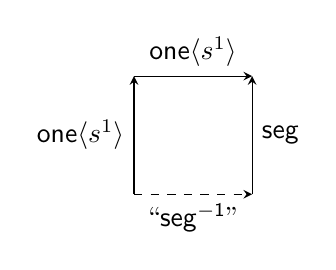
\begin{tikzpicture}[scale=.5]
    \draw[->,dashed,>=stealth] (0,0) -- (3,0) node [midway,below, fill=none] {``\cset{seg^{-1}}''};

    \draw[->,>=stealth] (0,3) -- (3,3) node [midway,above, fill=none] {\cont{\cset{one}}{\smap{1}}};
    \draw[->,>=stealth] (0,0) -- (0,3) node [midway,left, fill=none] {\cont{\cset{one}}{\smap{1}}};
    \draw[->,>=stealth] (3,0) -- (3,3) node [midway,right, fill=none] {\cset{seg}};
  \end{tikzpicture}
\end{center}

On the left and top side, the square is constantly \cset{one}. On the right hand
side, we have the \cset{seg} path. Then the bottom left corner of the square is
the 0-cell \cset{one} and the bottom right corner is \cset{zero}.
Kan composition of this open box gives us a cell with \cset{one} at its
left and \cset{zero} at its right boundary, which we could aptly call \cset{seg^{-1}}.

% TODO GOOD HERE?
% This principle has found its manifestation as a principle of logic. More general
% \cite{harper15_note_unifor_kan_condit_nomin_cubic_sets} by allowing multiple
% sides of the box to be missing and by also giving a filler for the whole cube,
% but this is not of concern for us in the following.

\todo{\cset{Int} is probably not the best motivating example. Can we find an example
  which feels more ``logical'' and is not directly related to homotopy theory?}

\paragraph{Poset maps as interval substitutions}

The above examples are common proof obligations in Cubical Agda. Searching for
interval substitutions automatically is difficult since it is not possible to
construct a formula of the distributive lattice by looking at the boundary which
needs to be filled (at least according to the author's knowledge). We 
will have to take a different perspective in the following, using a
correspondence between $n$-tuples of formulas in the free bounded distributive
lattice over $m$ elements and monotone
functions between the posets  $\{ 0<1 \}^m$ and $\{ 0<1 \}^n$.

% This correspondence is efficiently computable as we will see in
% \ref{sec:cubicalcorrespondence}, where we flash out the correspondence between
% our presentation and the one in Cubical Agda more concretely.


For example, the formula $i \vee j$ corresponds to the poset map $\{ 0<1 \}^2
\to \{ 0<1 \}^1$ which sends $00$ to $0$ and everything else to $1$. In our
setting, a cubical set
is a presheaf on the full subcategory of posets of the form $\{ 0<1 \}^n$, which
means that this poset map will be sent contravariantly to a map from the 1-cells
to the 2-cells of the cubical set. By filling in the definition of \cset{seg}
for the 1-cell, we can depict the action of the poset map on the 1-cell
\cset{seg} as follows:
\begin{center}
\begin{tikzpicture}
  % \node (zz) at (0,1) {\textcolor{gray}{00} $\mapsto \{x\}$};
  % \node (zo) at (-1,0) {\textcolor{gray}{01} $\mapsto \{x , y\}$};
  % \node (oz) at (1,0) {\textcolor{gray}{10} $\mapsto \{x , y\}$};
  % \node (oo) at (0,-1) {\textcolor{gray}{11} $\mapsto \{y\}$};
  \node (zz) at (0,1) {00};
  \node (zo) at (-1,0) {01};
  \node (oz) at (1,0) {10};
  \node (oo) at (0,-1) {11};
  \draw (zz) -- (zo) -- (oo) -- (oz) -- (zz);
  % \end{tikzpicture}
  % \begin{tikzpicture}[scale=1]
  \node (z) at (2.6,.7) {\cset{zero}};
  \node (o) at (2.6,-.7) {\cset{one}};
  \draw (z) -- (o) node[midway,right] {\cset{seg}};

  \draw[|->] (zz) -- (z);
  \draw[|->] (zo) -- (o);
  \draw[|->] (oz) -- (o);
  \draw[|->] (oo) -- (o);
\end{tikzpicture}
\end{center}

This depiction suggests a geometrical intuition for how the boundary of $\phi$
comes about: the faces $00-01$ and $00-10$ are the
\cset{seg} cell as $00$ is send to the left endpoint of \cset{seg} and $01$ and
$10$, respectively, to the right endpoint of \cset{seg}. The faces $01-11$ and $10-11$
are both constantly \cset{one} as both of its endpoints are send to the same
0-cell. This geometric intuition will allow us to find poset maps
efficiently, allowing us to construct cells that would have been forbidding to
find by brute-force.

Moreover, the poset map perspective allows us to gradually build open box to
find cells as Kan compositions.
\todo{MORNING derivation space perspective}

% The problem of whether a cell can be filled by
% Kan composition is in general undecidable, we will explore different semi-decidable
% procedures and heuristics to still come up with Kan compositions in many
% practical examples.


\paragraph*{Contributions and Structure}

The present paper is the first exploration of cubical sets from the point of
view of automated reasoning. We explore a presentation of cubical sets in terms of
presheaves on a certain category of posets and monotone maps and give a notion
of normal forms for cells of cubical sets in \autoref{sec:normalforms}. We
introduce the notion of potential poset maps as a useful data structure for
efficient search of poset maps in \autoref{sec:contortionsolver} and give an efficient
algorithm for finding poset maps for a given boundary.
We then extend our considerations to Kan cubical sets and establish why searching for
cells in Kan cubical sets is in general undecidable. We present efficient heuristics for
finding Kan compositions in many practical cases in
\autoref{sec:compositionsolver}. The findings of this paper have been used to
implement a tactic for Cubical Agda which we will discuss alongside a case study
deriving the Eckmann-Hilton argument in Cubical Agda TODO HOPEFULLY! in
\autoref{sec:cubicalagda} before concluding with some remarks in
\autoref{sec:conclusions}.


\section{Cubical Sets and Contortions}
\label{sec:normalforms}

In this section we will introduce the universe of discourse for our
considerations. We will define cubical sets and introduce some running examples
in \autoref{ssec:cubicalsets}. For proof search we require a finitary
representation of cubical sets, which mirror higher inductive types in Cubical
Agda and will be introduced in \autoref{ssec:hits}. We need a unique description for each cell of
a cubical set and introduce certain normal forms for this purpose in
\autoref{ssec:normalforms}.

\subsection{Cubical sets}
\label{ssec:cubicalsets}

The Dedekind cube category $\dedekind$ is the full subcategory of the category
of posets and monotone maps with objects $\pint{n}$ for $n \geq 0$, where $\pint{}
= \{ \izero < \ione \}$. Therefore morphisms in $\dedekind$ are of
the form $\pint{m} \to \pint{n}$. The cardinality of $\hom{\pint{m}}{\pint{}}$ is the
$m$-th Dedekind number, which explains the name of $\dedekind$.

We denote elements of $\pint{n}$ with $(e_1 \ldots e_n)$ where $e_i \in
\{\izero, \ione\}$ for $1 \leq i \leq n$ (we sometimes may omit the brackets).
For an element $x = (e_1 \ldots e_n)$ write $x_i \mdef e_i$. The poset
$\pint{0}$ has one element $()$. We will write $\pintrestr{n}{i}{e} \mdef
\{ x \in \pint{n} \mid x_i = e \}$, which is a subposet of $\pint{n}$.

\begin{definition}
Cubical sets are objects of $\psh{\dedekind}$, i.e., presheaves over the
Dedekind cube category.
\end{definition}

For a cubical set $X$ write $X_n \mdef X(\pint{n})$,
which are called the $n$-cells of $X$. Given an element $p$ of $X_n$, call
$\dim{p} \mdef n$ the dimension of $p$.

Given an $n$-cell $p$, any poset map $\sigma : \pint{m} \to \pint{n}$ gives rise to an $m$-cell
$X(\sigma)(p)$. We will write $\cont{p}{\sigma} \mdef X(\sigma)(p)$ and call
$\cont{p}{\sigma}$ an \mname{$m$-contortion} of $p$. We call $p$ the \mname{origin}
of $\cont{p}{\sigma}$ and refer to $n$ as the \mname{original dimension} of
$\cont{p}{\sigma}$. When restricting a function $\sigma$ to
$\pintrestr{m}{i}{e}$, we may freely use $\pint{m}$ or $\{ (x_1 ... x_{i-1}x_i
... x_n ) \mid x \in \pint{m} \}$ as a domain of $\restrict{\sigma}{\pintrestr{n}{i}{e}}$.

Certain poset maps of interest are:
\begin{align*}
  \smap{i} &: \pint{n} \to \pint{n-1}, (e_1 \ldots e_n) \mapsto (e_1 \ldots e_{i-1} e_{i+1} \ldots e_n) \text{ for } 1 \leq i \leq n\\
  \dmap{i}{e} &: \pint{n-1} \to \pint{n}, 
                (e_1 \ldots e_{n-1}) \mapsto (e_1 \ldots e_{i-1} e e_{i+1} \ldots e_{n-1}) \text{ for } 1 \leq i \leq n, e \in \{\izero,\ione\}
\end{align*}

Given an $n$-cell $p$, $\cont{p}{\smap{n+1}}$ is called a \mname{degeneracy} of
$p$. Given an $m > n$, we will write $\smap{m}$ for the composite
$\smap{n} \circ \smap{n+1} \circ \ldots \circ \smap{m}$. This gives the shorthand
$\cont{p}{\smap{m}}$ for $p$ considered as a degenerate $m$-cell.

Conversely, the cell $\cont{p}{\dmap{i}{e}}$ is called the $(i,e)$-th face of $p$. We
will call the list of all faces of an $n$-cell $p$ its boundary $\boundary{p}$:
$$\boundary{p} \mdef \mlist{ \cont{p}{\dmap{1}{\izero}},
  \cont{p}{\dmap{1}{\ione}} , \ldots , \cont{p}{\dmap{n}{\izero}}, \cont{p}{\dmap{n}{\ione}} }$$

% TODO extend definition of faces?
% - also include faces of faces, i.e., make ``congruence'' closure of faces
% - make it non-reflexive. We do not want that a cell is a face of itself since
% then normal form definition needs to be changed.

Contravariance in our cubical set means that for an $n$-cell $p$ and poset maps
$\sigma : \pint{m} \to \pint{n}$ and $\tau : \pint{l} \to \pint{m}$ we have 
$\cont{\cont{p}{\sigma}}{\tau} \mdef \cont{(\cont{p}{\sigma})}{\tau} =
\cont{p}{\sigma \circ \tau}$. For instance, we can use this to compute the
$(i,e)$-th face of a contorted cell with $\cont{\cont{p}{\sigma}}{\dmap{i}{e}} =
\cont{p}{\restrict{\sigma}{\pintrestr{n}{i}{e}}}$.

The central idea of this paper is the following: given some boundary, we want to
find a cell with this boundary. 
An $n$-dimensional boundary $T$ is a list of $2n$ cells $\mlist{p_{(1,\izero)},
  p_{(1,\ione)} , ... , p_{(n,\izero)}, p_{(n, \ione)}}$. We will write
$\boundaryface{T}{i}{e} \mdef p_{(i,e)}$.

\todo{Define valid boundary, i.e., state how cells in a boundary must be related}


\begin{example}\label{exp:int}
  The cubical set $\cset{Int}$ is generated by the following data: $\cset{Int}_0
  = \{ \cset{zero} , \cset{one} \}$ and $\cset{seg} \in \cset{Int}_1$ with
  $\cont{\cset{seg}}{\dmap{1}{0}} = \cset{zero}$ and $\cont{\cset{seg}}{\dmap{1}{1}} =
  \cset{one}$, which we could have written more concisely with
  $\boundary{\cset{seg}} = \mlist{\cset{zero}, \cset{one}}$.

  $\cset{Int}$ contains all necessary contortions, for instance
  $\cont{\cset{zero}}{\smap{1}}$ is a well-defined 1-cell which is
  degenerately $\cset{zero}$.
  The identity map gives an $n$-contortion for every $n$-cell which is equal
  to the original cell, for instance $\cont{\cset{seg}}{\oneid}$ is just the cell
  $\cset{seg}$.
\end{example}

\begin{example}\label{exp:sndsphere}
  We define the cubical set $\cset{Sphere}$ with the following data: We have a
  single 0-cell, so $\cset{Sphere}_0 = \{
  \cset{a} \}$. There is one non-degenerate 2-cell $\cset{\alpha} \in
  \cset{Sphere}_2$, which has a degenerate $\cset{a}$ for each of its faces,
  i.e.,
  $\boundary{\cset{\alpha}} = \mlist{ \cont{\cset{a}}{\smap{1}},
    \cont{\cset{a}}{\smap{1}}, \cont{\cset{a}}{\smap{1}}, \cont{\cset{a}}{\smap{1}} }$.
\end{example}

% \begin{example}\label{exp:torus}
%   We define the cubical set $\cset{Torus}$ with the following data: We have a
%   single 0-cell, so $\cset{Torus}_0 = \{ \cset{a} \}$. There are two
%   non-degenerate 1-cells $\cset{p}$ and $\cset{q}$ and one non-degenerate 2-cell
%   $\dmap{2}{0}(\cset{\alpha}) = \dmap{2}{1}(\cset{\alpha}) = p$ and
%   $\dmap{1}{0}(\cset{\alpha}) = \dmap{1}{1}(\cset{\alpha}) = q$.
% \end{example}

\begin{example}\label{exp:triangle}
  We define the cubical set $\cset{Triangle}$ as generated by the following
  data: The 0-cells are $\cset{Triangle}_0 = \{ \cset{x} , \cset{y} , \cset{z}
  \}$. The non-degenerate 1-cells are $\{ \cset{p} ,
  \cset{q} , \cset{r} \} \subseteq \cset{Triangle}_1$ with boundaries
  $\boundary{\cset{p}} = \mlist{ \cset{x} , \cset{y}}$
  $\boundary{\cset{q}} = \mlist{ \cset{y} , \cset{z}}$
  $\boundary{\cset{r}} = \mlist{ \cset{x} , \cset{z}}$.
  We have one non-degenerate 2-cell $\cset{\phi} \in \cset{Triangle}_2$ with
  $\boundary{\cset{\phi}} = \mlist{\cset{p} , \cset{r} , \cont{\cset{x}}{\smap{1}}  ,\cset{q}}$.
    % $\dmap{1}{0}(\cset{p}) = \cset{x}$ and $\dmap{1}{1}(\cset{p}) = \cset{y}$,
    % $\dmap{1}{0}(\cset{q}) = \cset{y}$ and $\dmap{1}{1}(\cset{q}) = \cset{z}$,
    % $\dmap{1}{0}(\cset{r}) = \cset{x}$ and $\dmap{1}{1}(\cset{r}) = \cset{z}$.
    % We have one non-degenerate 2-cell $\cset{\phi} \in \cset{Triangle}_2$ with $\dmap{1}{0}(\cset{\phi}) =
    % \cset{p}$, $\dmap{1}{1}(\cset{\phi}) = \cset{r}$, $\dmap{2}{0}(\cset{\phi})
    % = \smap{1}(\cset{x})$ and $\dmap{2}{1}(\cset{\phi}) = \cset{q}$.
\end{example}


% \begin{example}{\label{exp:assoc}}
%   Associativity of three paths
% \end{example}


\subsection{Higher inductive types}
\label{ssec:hits}

Cubical sets as introduced in the previous section are infinite objects:
as soon as there is a single cell in a cubical set $X$, we have faces or
degeneracies in all dimensions, and more generally all sorts of cells induced by
the poset maps. In order to mechanically search for cells in a cubical set, we
need a finitary representation of cubical sets. The examples above suggest that
we only require a bit of generating data from which the other cells and maps can
be inferred in a unique way.

% TODO BACKGROUND This is what HITs are for In
% \cite[Sect. 6.4]{bezem14_model_type_theor_cubic_sets}, strict groupoid turned
% into cubical set with general construction Higher inductive types are
% constructed as generalized pushout construction (free $\omega$-groupoid
% construction)


\begin{definition}
  A \mname{context} $\Gamma$ is a list of declarations $\mlist{ p_1 : T_1 ,
    \ldots , p_k : T_k}$ where each $T_j$ is a valid boundary using only
  contortions of cells $p_i$ with $i < j$. The cubical set $X$ generated by a context $\Gamma$
  has cells $p_i$ with boundaries $\boundary{p_i} = T_i$ for $1 \leq i \leq k$
  and all necessary other cells. We call $\ctxtdim{\Gamma} \mdef k$ the length
  of the context.
\end{definition}

% \todo{Define validity of boundary and context descriptions and give algorithm
%   checking validity.
  % Checking that a context is well-formed can be done in $\mathcal{O}(? k)$ and is
  % implemented in \autoref{alg:wellformedboundary} and
  % \autoref{alg:wellformedcontext}.
% }

\begin{examplecontd}{exp:int}
  The following context generates $\cset{Int}$:
  
  $\mlist{ \cset{zero} : \mlist{} , \cset{one} : \mlist{} , \cset{seg} : \mlist{
      \cont{\cset{zero}}{}, \cont{\cset{one}}{} }}$
\end{examplecontd}

\begin{examplecontd}{exp:sndsphere}
  The following context generates $\cset{Sphere}$:

  $\mlist{ \cset{a} : \mlist{} , \cset{\alpha} : \mlist{ \cont{\cset{a}}{\oneconst} , \cont{\cset{a}}{\oneconst} ,
  \cont{\cset{a}}{\oneconst}, \cont{\cset{a}}{\oneconst} }}$
  
\end{examplecontd}

\begin{examplecontd}{exp:triangle}
  The following context generates $\cset{Triangle}$:
  
  % $\mlist{ \cset{x} : \mlist{} , \cset{y} : \mlist{} , \cset{z} : \mlist{} ,
  %     \cset{p} : \mlist{ \cont{\cset{x}}{}, \cont{\cset{y}}{} } ,
  %   , \cset{q} : \mlist{ \cont{\cset{y}}{}, \cont{\cset{z}}{} }
  %   , \cset{r} : \mlist{ \cont{\cset{x}}{}, \cont{\cset{z}}{} }
  %   , \cset{\phi} : \mlist{ \cont{\cset{p}}{\oneid} , \cont{\cset{r}}{\oneid} ,
  %     \cont{\cset{x}}{\oneconst}, \cont{\cset{q}}{\oneid} }
  % }$

  $\mlist{ \cset{x} : \mlist{} , \cset{y} : \mlist{} , \cset{z} : \mlist{} ,
    \cset{p} : \mlist{ \cset{x}, \cset{y}  } ,
    , \cset{q} : \mlist{ \cset{y}, \cset{z} }
    , \cset{r} : \mlist{ \cset{x}, \cset{z} }
    , \cset{\phi} : \mlist{ \cset{p} , \cset{r} ,
      \cont{\cset{x}}{\oneconst}, \cset{q} }
  }$

\end{examplecontd}


In the following we will assume a valid context $\Gamma$
generating a cubical set $X$.


\subsection{Normal forms of contortions}
\label{ssec:normalforms}

There are different ways of describing a cell in a cubical set,
for instance , both $\cont{\cset{zero}}{\oneconst}$ and
$\cont{\cset{seg}}{\substtwo{0}{0}}$ in \autoref{exp:int} describe the same cell, namely the degenerate
1-cell which is constantly $\cset{zero}$. For our
considerations we will want a unique representation for every cell to allow for
literal comparisons between cells.

\begin{definition}
  A contortion $\cont{p}{\sigma}$ is in normal form if there is no
  $\cont{q}{\tau}$ such that $\cont{p}{\sigma} = \cont{q}{\tau}$ and $\dim{q} < \dim{p}$.
\end{definition}


We can efficiently compute the normal form of a contortion with
\autoref{alg:normalize}. Given a contortion $\cont{p}{\sigma}$,
we check whether $\sigma$ sends all elements of $\pint{m}$ to a
subposet $\pintrestr{n}{i}{e}$ of $\pint{n}$, which means that the contortion in
fact only talks about a face of $p$. If this is not the case we already
have been given a normal
form. Otherwise, we retrieve the $(i,e)$-th face of $p$, which we call $q$, and
normalize $q$ with the composed contortion.


\begin{algorithm}[H]
  \caption{Normalizing a contortion}
  \label{alg:normalize}
  \begin{algorithmic}[1]
    \Require $\cont{p}{\sigma}$ where $p : T \in \Gamma$ is an $n$-cell and
    $\sigma : \pint{m} \to \pint{n}$ \Ensure Normal form of $\cont{p}{\sigma}$

    \Procedure{Normalize}{$\cont{p}{\sigma}$}
    \If{$\exists 1 \leq i \leq n, e
      \in \{\izero, \ione\} : \image{\sigma} \subseteq \pintrestr{n}{i}{e}$}
    \State $\cont{q}{\tau} \gets \cont{p}{\dmap{i}{e}}$
    \State \Return{$\Call{Normalize}{\cont{q}{\tau \circ s^i \circ \sigma }}$ }
    \Else{}
    \State \Return{$\cont{p}{\sigma}$}
    \EndIf
    \EndProcedure

  \end{algorithmic}
\end{algorithm}

The algorithm is correct by the following reasoning: For a poset map $\sigma :
\pint{m} \to \pint{n}$ which satisfies for some $1 \leq i \leq n$, $e \in
\{\izero, \ione\}$ that $\sigma(x)_i = e$ for all $x \in \pint{m}$, we naturally
have $\sigma = \dmap{i}{e} \circ \smap{i} \circ \sigma$.
But then we have by functoriality for $\cont{q}{\tau} \mdef \cont{p}{\dmap{i}{e}}$:
$$\cont{p}{\sigma} = \cont{p}{\dmap{i}{e} \circ \smap{i} \circ \sigma} =
\cont{\cont{p}{\dmap{i}{e}}}{\smap{i} \circ \sigma} =
\cont{\cont{q}{\tau}}{\smap{i} \circ \sigma} = \cont{q}{\tau \circ \smap{i} \circ \sigma}$$

% This map comes about as follows: we
% know that  $\sigma(x)_i$ is the same for all $x \in \pint{m}$, so we can obtain
% $\cont{p}{\sigma}$ also as a contortion of $q$ by first applying $\sigma$, then
% forgetting about index $i$ with $s^i$ and finally applying the contortion
% of the face, $\sigma'$.

% TODO MORE EXPLANATION ABOUT HOW POSET MAPS ARE REPRESENTED AS DATA?
% Note that we can list elements of a poset
% such that if $x \leq y$ then $x$ is earlier than $y$ in the
% list. This allows us to traverse through the graph of a poset map and know that if an element
% $x$ is at a certain position in the list, all elements below $x$ will be seen at
% a certain point.

If we compute $\image{\sigma}$ as a multiset, checking whether 
$\image{\sigma}$ only contains elements of $\pintrestr{n}{i}{e}$ for
some $1 \leq i \leq n$ and $e \in \{\izero,\ione\}$ takes $\mathcal{O}(2^mn)$
(go through all $n$ indices of all $2^m$ elements of $\image{\pint{m}}$ and
return the first index at which all elements are the same, if there is such an index).
Since the dimension of the contortion under question is decreased by 1 in each
normalization step, we need to run the algorithm at most $n$ times and therefore
have a total complexity of $\mathcal{O}(2^mn^2)$ for contortion normalization.

\begin{examplecontd}{exp:triangle}
  The contortion $\cont{\phi}{\substfour{00}{00}{01}{01}}$ has normal form $\cont{p}{\substfour{0}{0}{1}{1}}$.
\end{examplecontd}

It is worth pointing out that contortions do not necessarily have unique boundaries.

\begin{examplecontd}{exp:sndsphere}
  Consider $T = \mlist{ \cont{\cset{a}}{\smap{1}} , \cont{\cset{a}}{\smap{1}}
    , \cont{\cset{a}}{\smap{1}} , \cont{\cset{p}}{\substtwo{00}{11}} }$.
  Both $\cont{\cset{p}}{\substfour{00}{00}{01}{11}}$ and
  $\cont{\cset{p}}{\substfour{00}{00}{10}{11}}$ are cells with boundary $T$.
\end{examplecontd}



% TODO GIVE EXAMPLE?
% (Term "a" (constSubst 1), Term "a" (constSubst 1) ) ,
% (Term "a" (constSubst 1), Term "p" (Map.fromList [(Vert [e0] , Vert [e0,e0]) , (Vert [e1] , Vert [e1,e1])]) )]
% solvable with 
%   (Vert [e0, e0] , [Vert [e0, e0]])
% , (Vert [e0, e1] , [Vert [e0, e0]])
% , (Vert [e1, e0] , [Vert [e0, e1] , Vert [e1 , e0]])
% , (Vert [e1, e1] , [Vert [e1, e1]])


% Disproved results

% \begin{proposition}
%   Uniqueness of contortions: if $\boundary{\cont{p}{\sigma}} =
%   \boundary{\cont{p}{\tau}}$ TODO ABOVE WITHOUT boundary, then $\sigma = \tau$.
% Nope. for instance for sphere we have several poset maps giving rise to
% [a<s1>, ... , ]
% \end{proposition}

% \begin{proposition}
%   If $\cont{p}{\sigma}$ is in normal form for $\dim{p} = n$ and $\sigma :
%   \pint{m} \to \pint{n}$ with $m > n$, then there is a face $\cont{p}{\tau}$ of
%   $\cont{p}{\sigma}$ (with $\tau : \pint{m-1} \to \pint{n}$).
% Nope. Have boundary of phi contortion which has only f and g by sending 0..0
% to 00, 1..1 to 11 and rest to 01.
% \end{proposition}



% \todo{where to describe \autoref{alg:boundary} }

% TERM DEFINITION 
% Given a context $\Gamma$, the set of $m$-dimensional terms over $\Gamma$, denoted $Tm_m(\Gamma)$, consists of
% \begin{itemize}
% \item Contortions $\cont{p}{\sigma}$ with $p \in \Gamma$ and $\sigma : \pint{m} \to
%   \pint{\dim{p}}$
%   % \item Kan compositions, i.e., $\comp{[(t_1 , s_1) , (t_m, s_m)]}{t}$ for all
% \item Kan compositions, i.e., $\comp{[t_1 , s_1, ... , t_m, s_m]}{t}$ for all
%   fitting $m$-contortions $t_1 , s_1, ... , t_m, s_m, t$.
% \end{itemize}


\section{Searching for Contortions}
\label{sec:contortionsolver}

In this section, we will study the following search problem: given a cubical set
and a certain boundary, we want to decide whether there is a cell in this
cubical set with that boundary. We will set out this problem in more detail in
\autoref{ssec:cubicalcell}. For our algorithms we introduce the notion of
potential poset maps which are introduced in \autoref{ssec:ppm} and use them to
devise an efficient algorithm for computing contortions in
\autoref{ssec:contortionsolver}. 


\subsection{The problem \myproblem{CubicalCell}}
\label{ssec:cubicalcell}

Using the finitary representation of cubical sets introduced in \autoref{ssec:hits}, we can phrase the problem of
finding a cell with a given boundary as follows:

\begin{definition}
  Given a context $\Gamma$ and a boundary $T$, the problem
  \myproblem{CubicalCell}($\Gamma$,$T$) is to find a cell $\cont{p}{\sigma}$ in
  the cubical set generated by $\Gamma$ such that
  $\boundary{\cont{p}{\sigma}} = T$.
\end{definition}

The problem \myproblem{CubicalCell} is clearly decidable since there are
only finitely many cells in a context which all have finitely many contortions
in a given dimension.
Hence, given an $m$-dimensional boundary $T$, we can go through all generators $p$
of the context and check whether a poset map $\pint{m} \to \pint{\dim{p}}$ gives
rise to $T$. However, the number of such poset maps 
grows super-exponentially: suppose we want to find an
$m$-dimensional contortion of a 1-cell, i.e., we are looking for a poset map
$\pint{m} \to \pint{}$. The number of such monotone maps is the $m$-th Dedekind
number, which we will denote $D_m$. For $m = 6$, we already have $D_6 = 7828354$
poset maps, and for 9 the exact number of possible poset maps is unknown
\footnote{\url{http://oeis.org/A00372}}. The number of such poset maps grows
furthermore exponentially with the dimension of original cell,
i.e., we have $D_m^n$ many monotone maps $\pint{m} \to \pint{n}$. 
Therefore searching for contortions by brute-force gets quickly infeasible and we
require something more clever to explore the search space.

% A certainly decidable subproblem of \myproblem{CubicalCell} is to decide whether
% there exists a cell simply by means of contorting the cells given in the
% context: for a given goal boundary $T$ and a generating cell $p$, there are
% finitely many poset maps $\pint{\dim{T}} \to \pint{\dim{p}}$, so we can
% na\"ively check whether one of those maps gives rise to a fitting contortion. 

% We can try this for all elements in the context, thereby have run time
% $\mathcal{O}( \ctxtdim{\Gamma} )$



% \subsection{General complexity considerations}
% Revert characterization 
% $$\dmap{i}{e}(X(\sigma)(p)) = X(\restrict{\sigma}{\pintrestr{n}{i}{e}})(p)$$
% TODO WHAT DID I MEAN BY THIS


\subsection{Potential poset maps}
\label{ssec:ppm}

For the following algorithms we introduce the notion of a potential poset map. In
essence, a potential poset map keeps track of all the values that elements of
the domain of the poset map could take, while making sure that there are no
superfluous values that cannot be part of any poset map as they would otherwise
violate monotonicity. Thereby we can represent all maps $\pint{m} \to \pint{n}$
at once with little data.

\begin{definition}\label{def:ppm}
  % A \mname{potential poset map} (\mname{ppm}) is a map $\Sigma : \pint{m} \to \pow{\pint{n}}$
  % such that for all $x \leq y$ : for all $u \in \Sigma(x)$ exists $v \in
  % \Sigma(y)$ such that $u \leq v$. TODO MORE

  A \mname{potential poset map} (\mname{ppm}) is a map $\Sigma : \pint{m} \to \pow{\pint{n}}$
  such that $\forall x \leq y$:
  \begin{itemize}
  \item $\forall u \in \Sigma(y) : \exists v \in \Sigma(x) : v \leq u$.
  \item $\forall v \in \Sigma(x) : \exists u \in \Sigma(y) : v \leq u$.
  \end{itemize}

\end{definition}

The two conditions above mean that any possible value in a ppm will give
rise to at least one poset map. TODO EXPLAIN WHY TODO TOTAL PPM TODO NON-EMPTY PPM


We will extend the notion of a contortion as a poset map applied to a cell to
also incorporate potential poset maps, leading to the notion of potential contortions.

\begin{examplecontd}{exp:int}
  Let us consider the potential contortion
  $\cont{\cset{seg}}{\substfour{\{0\}}{\{0, 1\}}{\{0, 1\}}{\{1\}}}$. To
  understand its action in the cubical set \cset{Int} we again fill in the
  definition of \cset{seg} into the poset map as follows:

  \begin{center}
      \begin{tikzpicture}[scale=.7]
        % \node (zz) at (0,1) {\textcolor{gray}{00} $\mapsto \{x\}$};
        % \node (zo) at (-1,0) {\textcolor{gray}{01} $\mapsto \{x , y\}$};
        % \node (oz) at (1,0) {\textcolor{gray}{10} $\mapsto \{x , y\}$};
        % \node (oo) at (0,-1) {\textcolor{gray}{11} $\mapsto \{y\}$};
        \node (zz) at (0,1) {$00$};
        \node (zo) at (-1,0) {$01$};
        \node (oz) at (1,0)  {$10$};
        \node (oo) at (0,-1) {$11$};
        \draw (zz) -- (zo) -- (oo) -- (oz) -- (zz);
        % \end{tikzpicture}
        % \begin{tikzpicture}[scale=1]
          \node (z) at (2.6,.7) {\cset{zero}};
          \node (o) at (2.6,-.7) {\cset{one}};
          \draw (z) -- (o) node[midway,right] {\cset{seg}};

          \draw[|->] (zz) -- (z);
          \draw[|->] (zo) -- (z);
          \draw[|->] (zo) -- (o);
          \draw[|->] (oz) -- (o);
          \draw[|->] (oz) -- (z);
          \draw[|->] (oo) -- (o);
      \end{tikzpicture}
    \end{center}

  % \vspace{1em}
      The ppm can be unfolded into four poset maps as we can choose the values
      of $01$ and $10$ independently. The squares resulting from using these
      poset maps for contortions of \cset{seg} are depicted below:

      \filledsquare{\cset{seg}}{\cset{seg}}{}{}{\substfour{0}{0}{1}{1}}
      \filledsquare{\phantom{\cset{seg}}}{\phantom{\cset{seg}}}{\cset{seg}}{\cset{seg}}{\substfour{0}{1}{0}{1}}
      \filledsquare{\cset{seg}}{\phantom{\cset{seg}}}{\cset{seg}}{}{\substfour{0}{1}{1}{1}}
      \filledsquare{\phantom{\cset{seg}}}{\cset{seg}}{}{\cset{seg}}{\substfour{0}{0}{0}{1}}

      All these contortions have in common that the bottom left corner is
      \cset{zero} and the top right corner is \cset{one}, which we could already
      read off from the potential contortion.

\end{examplecontd}

Thereby ppms are a useful notion to capture a number of poset maps with
little data. For example, representing all $D_n$ poset maps $\pint{n} \to
\pint{}$ requires only $2^n$ entries of $\{0,1\}$. Our goal in the following
will be to restrict a ppm until only few poset maps remain. We can unfold a ppm $\Sigma$
into the set of poset maps that it is representing with the procedure
$\Call{UnfoldPPM}{\Sigma}$ given in \autoref{alg:getsubsts} in the appendix. If we
want to narrow down a ppm to take values $vs \subseteq \Sigma(x)$ for some $x$, we can
update it in $\mathcal{O}(2^m2^n)$ to still satisfy the conditions in
\autoref{def:ppm} with the algorithm \autoref{alg:updateppm}.

% A non-empty ppm is one which has a non-empty set of possible values
% for any element, which can be checked in $2^m$ steps.

% Given a poset $xs
% \subseteq \pint{m}$, we can restrict a ppm $\Sigma : \pint{m} \to \pow{\pint{n}}$ to a
% new ppm $\restrict{\Sigma}{xs} : xs \to \pow{\pint{n}}$ just like any function.


\subsection{Contortion solver}
\label{ssec:contortionsolver}

Using the notion of potential poset maps, we develop in this section an
efficient algorithm for deciding whether a cell $p$ can be contorted into a given
boundary $T$. The central idea is that we start with a total ppm and gradually
narrow it down by looking at the faces of $T$ in descending original dimension.
The algorithm is given in \autoref{alg:simple}.

\begin{algorithm}[H]
  \caption{Contortion solver}\label{alg:simple}
  \begin{algorithmic}[1]
    \Require $\Gamma$ context, $p \in \Gamma$, $T$ goal boundary with $n \mdef \dim{p} , m \mdef \dim{T} $
    \Ensure $\sigma : \pint{m} \to \pint{n}$ s.t. $\boundary{\cont{p}{\sigma}} = T$ if there is such a
    $\sigma$, \texttt{Unsolvable} otherwise

    \Procedure{ContortionSolve}{$p$} % TODO WHICH INPUT
    \State $\Sigma \gets \{ x \mapsto \pint{n} \mid x \in \pint{m} \}$ \label{cont:line:initsigma}
    \For{$\cont{q}{\tau} \mdef \boundaryface{T}{i}{e} \text{ with } i \gets \{1 ,... , m\}, e \gets \{\izero,
      \ione\}$ such that $\dim{q} $ desc.}
    % \For{$i \gets 1\leq i \leq m, e \gets \{\izero, \ione\}$}
    \If{$p = q$}
      \State $\Theta \gets \{ x \mapsto \tau(x) \mid x \in \pintrestr{m}{i}{e}
      \}$ \label{cont:line:peqq}
    \Else
      \State $\Theta \gets \{ x \mapsto \emptyset \mid x \in \pintrestr{m}{i}{e} \}$
      \For{$\sigma \gets
        \Call{UnfoldPPM}{\restrict{\Sigma}{\pintrestr{m}{i}{e}}}$} \label{cont:line:unfold}
        \If{$T_{i=e} = \Call{Normalize}{\cont{p}{\sigma}}$}
          \For{$x \in \pintrestr{m}{i}{e}$}
            \State $\Theta(x) \gets \Theta(x) \cup \{ \sigma(x) \}$
          \EndFor
        \EndIf
        \EndFor
        \EndIf
      \For{$x \in \pintrestr{m}{i}{e}$}
      \State \Call{UpdatePPM}{$\Sigma, x, \Theta(x)$} \label{cont:line:update}
      \EndFor
    \EndFor
    \If{$\exists \sigma \in \Call{UnfoldPPM}{\Sigma} :
      \boundary{\cont{p}{\sigma}} = T$} \label{cont:line:check}
      \State \Return{$\sigma $}
    \Else
    \State \Return{\texttt{Unsolvable}}
    \EndIf
    \EndProcedure
  \end{algorithmic}
\end{algorithm}

We first generate the most general ppm
$\Sigma$ in line \ref{cont:line:initsigma}. We then go through each face
$\cont{q}{\tau}$ of the goal boundary $T$ and use it to restrict $\Sigma$.
Crucially, we order the faces by their original dimensions as higher-dimensional
cells in the boundary will restrict $\Sigma$ more than lower-dimensional faces.

Given a face $\cont{q}{\tau}$, we proceed as follows: in case the face has the
same original cell as the cell we are contorting, we can give unique values for
all element of the subposet corresponding to the current face as done in line \ref{cont:line:peqq}.
Otherwise, we generate all possible faces that could be generated from $\Sigma$
at the subposet and only keep values that contributed to some valid face.
We finally propagate our findings through the whole poset map $\Sigma$ in line \ref{cont:line:update}.

After restricting $\Sigma$ according to all faces we generate a valid solution
and return it in line \ref{cont:line:check}.

\paragraph{Correctness}

The algorithm is cleary correct since we only return a poset map $\sigma$ if
it is indeed contorting $p$ to the correct boundary. Note that we have to do
this step as there might be multiple solutions. Since our ppms captures all
solutions at once, we need to make sure that we do not return assignments of
different solutions. TODO MAKE CLEARER, PERHAPS WITH EXAMPLE

\paragraph{Completeness}

Supposing that a cell exists with a boundary, we want to show that we find it.
This follows immediately since any value in the ppm contributing to some
solution has been kept. TODO ELABORATE

\paragraph*{Runtime}

The most expensive step in the algorithm is unfolding all poset maps of the
subposet in line \ref{cont:line:unfold}. In the worst case, we have $D_{m-1}^n$
many poset maps that we need to check, and as we are doing this for all $2m$
faces of $T$ we have a factor of $2 m D_{m-1}^n$ in the asymptotic runtime. After performing
all restrictions, $\Sigma$ is usually unique or contains very few poset maps,
which is why the unfolding step in line \ref{cont:line:check} is not expensive.

The algorithm constitutes an improvement over na\"ively checking all 
$D_m^n$ poset maps already in the worst case as the Dedekind
numbers grow quicker than any operation in our algorithm, and hence our
algorithm has a runtime which is one Dedekind number quicker than the na\"ive
algorithm. In many practical cases, the original face of the contortion
appears in its boundary, which significantly allows to reduce the search space
before any ppm is unfolded. This means that we can compute many contortions that
would have been impossible to find by brute-force.


\begin{examplecontd}{exp:sndsphere}

  We want to find
  $\sigma : \pint{3} \to \pint{2}$ such that $\cont{\alpha}{\sigma}$ has boundary
$T = \mlist{ \cont{\cset{\alpha}}{\substfour{00}{01}{01}{11}} ,
  \cont{\cset{a}}{\smap{2}} , \cont{\cset{a}}{\smap{2}} ,
  \cont{\cset{a}}{\smap{2}} , \cont{\cset{a}}{\smap{2}} ,
  \cont{\cset{a}}{\smap{2}}}$.

In the beginning, the total ppm $\Sigma$ is initialized with $\{ x \mapsto
\pint{2} \mid x \in \pint{3}\}$.
We then go through all faces of the goal boundary and use them to restrict
$\Sigma$.
The face of the boundary with the largest original dimension is a contortion of
$\alpha$. Since $\alpha$ is also the cell that we are contorting, the subposet
$\pintrestr{3}{1}{\izero}$ of the domain of $\Sigma$
is mapped in a unique way to the elements of $\pint{2}$. The monotonicity
restrictions on ppms further restrict $\Sigma$: since $011$ is mapped to the
bottom element $00$, also $111$ will need to be mapped to $00$. The elements
$101$ and $110$ lie below elements which are mapped to $01$, which mean that
there are only two possible values $\{01, 11\}$ for each of these elements. Only
the element $001$ has the full poset $\pint{2}$ as potential values. In summary,
we have the following potential contortion after the first restriction of $\Sigma$:
\begin{center}
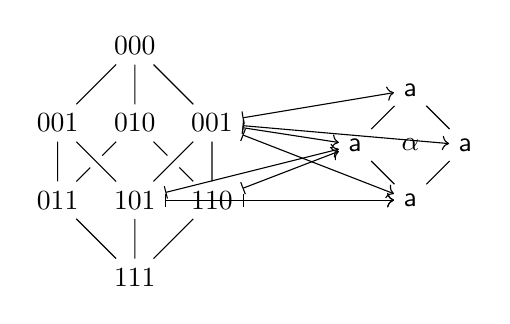
\begin{tikzpicture}[scale=.7]
      \node (zzz) at (0,2.8) {$000$};
      \node (zzo) at (-1.4,1.4) {$001$};
      \node (zoz) at (0,1.4) {$010$};
      \node (zoo) at (-1.4,0) {$011$};
    \node (ozz) at (1.4,1.4) {$001$};
    \node (ozo) at (0,0) {$101$};
    \node (ooz) at (1.4,0) {$110$};
    \node (ooo) at (0,-1.4) {$111$};
    \draw (ooo) -- (zoo) -- (zzo) -- (zzz) -- (zoz) -- (ooz)
    (ozo) -- (ooo) -- (ooz) -- (ozz) -- (zzz)
    (zoo) -- (zoz);
    \draw[preaction={draw=white, -,line width=6pt}] (zzo) -- (ozo) -- (ozz);

    \begin{scope}[shift={(5,1)}]
      \node (zz) at (0,1) {\cset{a}};
      \node (zo) at (-1,0) {\cset{a}};
      \node (oz) at (1,0) {\cset{a}};
      \node (oo) at (0,-1) {\cset{a}};
      \node (filler) at (0,0) {\cset{\alpha}};
      \draw (zz) -- (zo) -- (oo) -- (oz) -- (zz);
    \end{scope}

    \draw[|->] (ozo) -- (zo);
    \draw[|->] (ozo) -- (oo);
    \draw[|->] (ooz) -- (zo);
    \draw[|->] (ooz) -- (oo);
    \draw[|->] (ozz) -- (zz);
    \draw[|->] (ozz) -- (zo);
    \draw[|->] (ozz) -- (oz);
    \draw[|->] (ozz) -- (oo);
  \end{tikzpicture}
\end{center}

We then check for each of the faces which are degenerate \cset{a} whether
$\Sigma$ gives rise to such a face. Crucially, this will be done quickly as
there are only 10 poset maps in the ppm $\Sigma$ remaining after the restricting
$\Sigma$ according to the first face of $T$.

\end{examplecontd}



% \begin{algorithm}[H]
%   \caption{Simple solver recursively}\label{alg:simple}
%   \begin{algorithmic}
%     \Require $\Gamma$ context, $p \in \Gamma$, $T$ goal boundary ($n \mdef \dim{p} , m \mdef \dim{T} $)
%     \Ensure All $\sigma$ s.t. $\boundary{\cont{p}{\sigma}} = T$

%     \Procedure{SimpleSolve}{$p$}
%     \State $\Sigma \gets \{ x \mapsto \pint{n} \mid x \in \pint{m} \}$
%     \For{$i \gets 1\leq i \leq m, e \gets \{\izero, \ione\}$}
%       \State $\Theta \gets (x : \pintrestr{m}{i}{e} )\mapsto \emptyset$
%       \For{$\sigma \gets \Call{SimpleSolve}{\boundary{T_{i=e}}}$}
%         \For{$x \in \pintrestr{m}{i}{e}$}
%           \State $\Theta(x) \gets \Theta(x) \cup \{ \sigma(x) \}$
%         \EndFor
%         \EndFor
%         \For{$x \in \pintrestr{m}{i}{e}$}
%           \State \Call{UpdatePPM}{$\Sigma, x, \Theta(x)$}
%         \EndFor
%     \EndFor
%     \State \Return{$\{ \sigma \mid \sigma \in \Call{UnfoldPPM}{\Sigma} :
%     \boundary{\cont{p}{\sigma}} = T \}$}
%     \EndProcedure
%   \end{algorithmic}
% \end{algorithm}


% More than that, the potential substitutions allow us to narrow down the search
% space in other ways.

% Try to reduce the search space going from the bottom.



% \begin{examplecontd}{exp:sndsphere}
%   TODO UPDATE WITH NEW ALGORITHM
%   5-dimensional analogue of above cube is solved in  $< 5$ seconds.
%   Try out $\mathcal{O}(D_4^2 = 168^2 = 28224)$ poset maps for all 10 faces, combine all
%   fitting poset maps in ppm.
%   This ppm unfolds to 168 poset maps of type
%   $\pint{5} \to \pint{2}$, filter which one fits.

%   Brute force approach would require checking $D_5^2 = 7581^2 = 57,471,561$
%   poset maps.
% \end{examplecontd}






\section{Composition solver}
\label{sec:compositionsolver}

Cubical type theory is based on a certain class of cubical sets, namely those
that can model spaces. Kan \cite{kan55_abstr_homot} introduced a single
condition for this purpose, which essentially states that any open cube can be
filled in a coherent way. By turning cubical sets into a logic, cubical type
theory turns the Kan condition into a logical rule.


TODO STRUCTURE OF SECTION

\subsection{Kan cubical sets}

In essence, Kan composition establishes that if one constructs a valid cell
with only one face missing, then this face exists as well. For example, we can
invert the path \cset{seg} in \autoref{exp:int} by constructing an open square
as follows:

\begin{center}
\compsquare{\cset{seg}}{\cont{\cset{zero}}{\smap{1}}}{\cont{\cset{zero}}{\smap{1}}}{\cset{p}^{-1}}
\end{center}

TODO give p q composition

Let us make this more precise. We have the following notion of open cube, which
we call \mname{box}:
an $(n+1)$-dimensional box $U$ is a collection of $2 \cdot n + 1$ cells, which
we will write $\cbox{p_1 , q_2 , ... , p_n , q_n }{r}$. We call $r$ the back of
$U$, $p_i$ its $(i,0)$-th side and $q_i$ its $(i,1)$-th side.


\begin{definition}
  A Kan cubical set $X$ is cubical set which furthermore satisfies the following
  condition: given a box $U \mdef \cbox{p_1 , q_2 , ... , p_n , q_n }{r}$, $X$
  has the following cells:
  \begin{itemize}
  \item  $\ccomp{U}$ with boundary $\mlist{ \cont{p_1}{\dmap{n}{\ione}} ,
      \cont{q_1}{\dmap{n}{\ione}} , ... , \cont{p_n}{\dmap{n}{\ione}} ,
      \cont{q_n}{\dmap{n}{\ione}} }$, called the composition of $U$.
  \item  $\cfill{U}$ with boundary $\mlist{ p_1 , q_1 , ... , p_n , q_n , r ,
      \ccomp{U} }$, called the filler of $U$.
  \end{itemize}
\end{definition}

Note that cubical type theory as presented in \cite{cohen18_cubic_type_theor}
uses a more general Kan condition. We will not need this principle in this
generality and will use the above notion for the sake of concreteness. TODO
DISCUSS RELATION IN A BIT MORE DETAIL?

% With this we can make more complex definitions and include the composition and
% fillers of boxes in the boundary assignments of a cell.

% \begin{example}\label{exp:s3}
%   The Kan cubical set \cset{S3} contains a single 0-cell $\star$, two 1-cells $a$
%   and $b$ and three 2-cells $\boundary{\cont{\star}{\smap{1}} ,
%     \cont{\star}{\smap{1}} , \cont{\star}{\smap{1}} , w }$ for $w \in \{ aaa ,
%     bb , abab\}$
%   \end{example}



\subsection{Undecidability of finding cells in a Kan cubical set}
\label{ssec:kanundecidable}

Since the cells of a box can itself be the result of composing or filling a box,
the search space for Kan cubical cells grows infinitely large. Naturally,
deciding whether there is a cell in a Kan cubical set with a specific boundary
is undecidable, which we will demonstrate in this section with a reduction to
string rewrite systems.

The problem of finding cells in a Kan cubical set is the following:

\begin{definition}
  Given a context $\Gamma$ and a boundary $T$, the problem
  \myproblem{KanCubicalCell}($\Gamma$,$T$) is to find a cell $p$ in the Kan cubical
  set generated by $\Gamma$ such that $\boundary{p} = T$.
\end{definition}

We can encode very many structures and problems with Kan cubical sets: groups,
... TODO GIVE OVERVIEW.

\begin{proposition}
  \myproblem{KanCubicalCell} is undecidable.
  \begin{proof} 
    We show how the word problem for Thue systems \myproblem{Word} reduces to
    \myproblem{KanCubicalCell}. Given a Thue system $(\Sigma,R)$ consisting
    of an alphabet $\Sigma$ and a symmetric relation over words of $\Sigma$, $R \subseteq
    \Sigma^* \times \Sigma^*$. The rewriting relation is defined as follows: we
    have $s \to_R t$ if there are $x,y,u,v \in \Sigma^*$ such that $s=xuy$,
    $t=xvy$ and $(u,v) \in R$.

    We construct the following cubical set. We have a single 0-cell $\star$, 1-cells $\Sigma$ and for any
    $(u,v) \in R$ a 2-cell $r_{u,v}$ with $\boundary{r_{u,v}} = \mlist{
      u, v , \cont{\star}{\smap{1}},
      \cont{\star}{\smap{1}} }$ where we use path composition TODO WHERE
    INTROCED AND SHOWN ASSOC for concatenating letters and $\cont{\star}{\smap{1}}$ as the empty
    word.

    The reflexive transitive closure of the rewriting relation, denoted $s
    \to_R^* t$, is mirrored in the Kan cubical set as follows: for any $s$, we
    have a proof of reflexivity $\cont{s}{\smap{2}}$. Suppose we have a cell $A$
    witnessing $u \to_R^* v$, then the following cell witnesses that $s = xuy
    \to_R^* xvy=t$:

    \begin{center}
      \hcompcube{\cont{\star}{\smap{1}}}{\cont{\star}{\smap{1}}}{t}{s}{\cont{x}{\smap{2}}}{\cont{y}{\smap{2}}}{.fill}{.fill}{A}
    \end{center}

    TODO SPELL OUT CONNECTION IN MORE DETAIL

    Therefore any rewriting sequence between two words $u$ and $v$ 
    corresponds precisely to a 2-dimensional cell with boundary
    $\mlist{u,v,\cont{\star}{\smap{1}} , \cont{\star}{\smap{1}}}$. If it was
    decidable whether such a cell exists, we would have a decision procedure for
    \myproblem{Word}.
    

    % Given a group $G$ generated by $\langle A \mid R \subseteq A^* \rangle$,
    % i.e., elements of $G$ are words $a_1 ... a_n \in A^*$ with neutral
    % element $e$, and any relation $r \in R$ means that $r = e$ in the group.
    % % $X$, i.e., $R \subseteq \{ a_1 \mathellipsis a_n \mid a_\_ \in X \cup X^{-1}
    % % \}$ such that for all $w \in R$, we have $w = e$ in $G$.

    % Construct the cubical set \cset{G} with 0-cell $\star$, 1-cells $A$ with
    % $\boundary{a} = \mlist{\star , \star}$ for any $a \in A$, and for each $r \
    % \in R$ a 2-cell $r$ with $\boundary{r} = \mlist{ \cont{\star}{\smap{1}} ,
    %   \cont{\star}{\smap{1}} , \cont{\star}{\smap{1}} , r}$. This means we use Kan
    % composition as the group operation and the reflexive path on $\star$ as the
    % neutral element.

    % % \todo{We need to have introduced compositions as this point}
    % % \todo{We need to have introduced inverses as this point}

    % The word problem for groups is now the following: given a word $w \in A^*$,
    % is $w = e$. We claim that if \myproblem{KanCubicalCell} was decidable, we
    % could decide whether $w = e$.

    % Recall that $w = e$ holds precisely if one of the following conditions hold:
    % \begin{itemize}
    % \item $w = uv$ and $u = e$ and $v = e$
    % \item $w = u aa^{-1}v $ or $w = ua^{-1}av $ and $uv = e$
    % \item we have $a^{-1}wa = e$ or $awa^{-1} = e$
    % \end{itemize}

    % We will now show that these reduction rules are mirrored by 2-cells in
    % \cset{G}.

    % Since path composition is associative, we have a filler for the following
    % cell

    % Suppose $w = uv$ (should we distinguish meta =?) Our induction hypothesis is that we have cells $\phi$ proving $u = e$ and
    % $\psi$ proving $v = e$. Then we have the following cell:

    % \hcompcube{\cont{\star}{\smap{1}}}{\cont{\star}{\smap{1}}}{\cont{\star}{\smap{1}}}{uv}{\cont{\star}{\smap{2}}}{\psi}{\cont{\star}{\smap{2}}}{.fill
    % u v}{\phi}


    % \hcompcube{i0}{i1}{j0}{uaa^{-1}v}{fi0}{fi1}{fj0}{fj1}{A}

    % TODO FOR OTHER TWO RULES

    % Hence if we were able to decide \problem{KanCubicalCell}, we could establish
    % whether such a cell exists and hence decide the word problem for an arbitrary group.


    % TEMPLATE \hcompcube{i0}{i1}{j0}{j1}{fi0}{fi1}{fj0}{fj1}{A}

    % Finitely generated: $X$ is finite
    % Finitely presented: $X$ and $R$ are finite

    % Given a set of generators $\{a, ...\}$ of a group $G$, define $\cset{Group}$
    % with a single 0-cell $\cset{Group}_0 = \{ \cset{\star} \}$, 
    % 1-cells $\{\cset{a} , \cset{a^{-1}} ... \} \subseteq \cset{Group}_1$ and a
    % 2-cell $\cset{idem_a}$ for any generator $a$ with 
    % $\dmap{2}{0}(\cset{idem_a}) = \cset{a}$, $\dmap{1}{1}(\cset{idem_a}) =
    % \cset{a^{-1}}$ and $\dmap{2}{1}(\cset{idem_a}) = \dmap{1}{0}(\cset{idem_a}) = \smap{1} (\cset{\star})$.

    % Given a set of generators $\{a, ...\}$ of a group $G$, define $\cset{Group}$
    % with a single 0-cell $\cset{Group}_0 = \{ \cset{\star} \}$, 
    % 1-cells $\{\cset{a} , ... \} \subseteq \cset{Group}_1$ 

    % (there are more 2-cells that need to be added as explained in \cite[Sect. 6.3]{bezem14_model_type_theor_cubic_sets})
    % % Note that this is not a set. Doesn't matter for undecidability proof?

    % \todo{Give reduction Word < KanCubicalCell. For some specific group with
    %   undecidable word problem or Uniform word problem? }
\end{proof}
\end{proposition}


\subsection{Finding Kan compositions using constraint satisfaction}

In order to find Kan compositions, we can use the language of constraint
satisfaction programming.

Given a HIT $X$

To construct an $n$-dimensional box whose composition has a given boundary $T$, we
have the following CSP:

\begin{itemize}
\item Variables $X_{\text{Back}}$ and $X_{(i,e)}$ for $1 \leq i \leq n$,
  $e\in\{\izero,\ione\}$ stand for the back and side faces of the cube.
\item $D_{\text{Back}} = \{ \cont{p}{TODO total sigma from n \to \dim{p}} \mid p \in X \}$
  and
  $D_{(i,e)} = \{ \cont{p}{TODO total sigma from n \to \dim{p}} \mid p \in X
  \text{ such that } \cont{p}{\dmap{\ione}{n}} = \boundaryface{T}{i}{e} \}$
\item Constraints are that all boundaries of the sides and back need to match.

  Back constraints: $\termface{X_{\text{Back}}}{i}{e} =
  \termface{X_{(i,e)}}{n}{\izero}$

  Side constraints: $\termface{X_{(i,e)}}{i}{e'} = \termface{X_{(i',e')}}{i}{e}$
  for $1 \leq i < j \leq n$ and $e,e' \in \{ \izero, \ione \}$.
\end{itemize}


When this does not work, we can create a larger CSP where one of the faces is
itself the result of a Kan composition. We cannot pass over results from the
1-dimensional case. Also not clear in which direction we need to extend our
cube. For the 1-dimensional cube we can however safely only extend in one direction.

\todo{EXTEND TO NESTED CUBES. EXAMPLE WITH PATH COMPOSITION}



% \section{Negation}

% How to encode search for reversals


\section{Case study: TODO}
\label{sec:cubicalagda}

We have reasoned about semantic objects in this paper: since syntax and semantics so
closely linked, this gives us a syntactic solver as well. We just have to
translate to the term language of Cubical Agda.

The above algorithms have been implemented in
\url{https://github.com/maxdore/cubetac/}. In the following we will discuss how
our approach relates to Cubical Agda and a case study using this tactic.


% As observed by \cite{orton17_axiom_model_cubic_type_theor_topos}, we do not require
% a full De Morgan structure. In particular, it suffices to consider only $\meet$
% and $\join$ forming a bounded free distributive lattice. Model structure open
% problem, but it is conjectured that it does.


\subsection{Connecting with Cubical Agda}

The morphisms in $\dedekind$ have a succinct description as tuples of formulas
of a free distributive lattices, these formulas are also used in Cubical Agda.
In order to use our algorithms in a tactic for Cubical Agda, we need to
translate back and forth efficiently between both characterizations of $\dedekind$.

To generate a lattice formula from a poset map we can use \autoref{alg:subst2tele}.

\begin{algorithm}[H]
  \caption{Poset map to lattice formula}\label{alg:subst2tele}
  \begin{algorithmic}
    \Require $\sigma : \pint{m} \to \pint{n}$
    \Ensure $\phi$ $n$-tuple of elements of free distributive lattice over $m$ variables

    \Procedure{Subst2Tele}{$\sigma$}
    \For{$i \gets 1$ to $n$} 
      \State $\phi_i \gets \{ x \in \pint{m} \mid \sigma(x)_i = 1 \}$
      \Comment{$\mathcal{O}(2^m)$ many elements in $\pint{m}$}
    \EndFor
    \State \Return{$(\phi_1, ... , \phi_n)$}
    \EndProcedure
  \end{algorithmic}
\end{algorithm}

Given $\sigma : \pint{m} \to \pint{n}$, we compute an $n$-tuple of elements of the
free distributive lattice over $m$ elements as follows:
The $i$-th entry is $\{ x \in \pint{m} \mid s(x)_i = 1 \}$. An element $x$ can be
seen as a clause if we regard it as indicator of which elements of the lattice
are used, e.g., $(1,0,1)$ represents the clause $x \meet z$ if the three
elements of the lattice are $x$, $y$ and $z$.

% TODO mention set representation of DNF. Also mention normalization necessary --
% what's its runtime?

For the converse we can use \autoref{alg:teletosubst}

\begin{algorithm}[H]
  \caption{Lattice formula to poset map}\label{alg:teletosubst}
  \begin{algorithmic}
    \Require $\phi$ $n$-tuple of elements of free distributive lattice over $m$ variables
    \Ensure $\sigma : \pint{m} \to \pint{n}$

    \Procedure{Tele2Subst}{$p$}
    \For{$x \gets \pint{m}$} 
      \For{$i \gets 1$ to $n$}
        \State $\sigma(x)_i \gets \phi_i @ x$
      \EndFor
    \EndFor
    \State \Return{$\sigma$}
    \EndProcedure
  \end{algorithmic}
\end{algorithm}

From an $n$-tuple of formulas over $\phi$ we can read off a poset map $\sigma :
\pint{m} \to \pint{n}$ as follows: Given an element $x \in \pint{m}$, $\sigma(x) = (e_1
, ... , e_n) $ where $e_i = \phi_i @ x$. Here $\phi_i$ is the $i$-th element of
the tuple $\phi$ and $@$ denotes evaluation of formulas: The indices of $x$
which are set to 1 mean that the corresponding variable of $\phi$ is ``true'',
then we check whether the formula evaluates in total to true by interpreting
join and meet as logical operations.

\todo{The above presentation is not very clean and should be streamlined.}

Therefore going back and forth between formulas and poset map takes
$\mathcal{O}(2^mn)$ many steps. This is linear in the number of elements of the
data structures we are considering, so does not pose an issue for performance of
our tactic.

% \begin{example}
%   % EXAMPLE
%   % [(000,00),(001,00),(010,00),(011,01),(100,10),(101,11),(110,10),(111,11)]
%   % 1 ((2 /\ 3) \/ (1 /\ 3))
% \end{example}

% TODO PROOF THAT THESE ARE MUTUALLY INVERSE?
\todo{Show correctness of both algorithms and that they are mutually inverse.}

Cubical Agda uses PathP types to represent boundaries of a cube. The PathP type
has three constructors, where the first is again a PathP type, allowing for
nesting paths and thereby creating higher cubes. If the second and third
parameter are $n$-dimensional paths, then the first parameter might introduce
$n$ interval variables.


\begin{examplecontd}{exp:sndsphere}
  
The proof goal already introduced above:

$$\mlist{ \cont{\cset{p}}{\substfour{00}{01}{01}{11}} ,
  \cont{\cset{a}}{\smap{2}} , \cont{\cset{a}}{\smap{2}} ,
  \cont{\cset{a}}{\smap{2}} , \cont{\cset{a}}{\smap{2}} ,
  \cont{\cset{a}}{\smap{2}}}$$

has the following corresponding PathP type in Cubical Agda.
  \begin{align*}
    \mathsf{PathP} (\lambda i \to \mathsf{PathP} &(\lambda j \to  \mathsf{Path} \ (\cset{p} \ (i \wedge
                                                   j) \ (i \vee j))\ \cset{a})\\
                                                 &(\lambda j \to \cset{a}) (\lambda j \to \cset{a}))
                                                   (\lambda i j \to \cset{a}) (\lambda i j \to \cset{a})
  \end{align*}
\end{examplecontd}

\todo{Translating between our notions and PathP types is straightforward, we
  should still explain it here}



% \subsection{Nominal perspective}

% Have set $I = \{i , j, k , ...\}$ of names. Then give complete description for
% Cubical Agda.


\section{Conclusions}
\label{sec:conclusions}

\todo{}

Check whether decidable subproblems: Only finitely many cells/ up to dim n/ ...?

% \addcontentsline{toc}{section}{References}

\bibliographystyle{plain}
\bibliography{bibliography}



\appendix

\begin{algorithm}[H]
  \caption{Update potential poset map}\label{alg:updateppm}
  \begin{algorithmic}
    \Require $\Sigma : \pint{m} \to \pow{\pint{n}}$ ppm, $x \in
    \pint{m}$, $vs \subseteq \Sigma(x)$ % $vs \in \pow{\pint{n}} - \emptyset$
    \Ensure Updated ppm $\Sigma' : \pint{m} \to \pint{n}$ with $\Sigma(x) = vs$.

    \Procedure{UpdatePPM}{$\Sigma, x,vs)$}
    \For{$y \gets \pint{m}$}
    \If{$x = y$}
    \State $\Sigma'(x) \gets vs$
    \ElsIf{$y \leq x$}
    \State $\Sigma'(y) \gets \{ u \mid u \in \Sigma(y) \text{ such that } \exists
    v \in vs : u \leq v \} $
    \ElsIf{$x \leq y$}
    \State $\Sigma'(y) \gets \{ u \mid u \in \Sigma(y) \text{ such that } \exists
    v \in vs : v \leq u \} $
    \EndIf
    \EndFor
    \State \Return{$\Sigma'$}
    \EndProcedure
  \end{algorithmic}
\end{algorithm}

TODO EXPLAIN
Worst case run-time of $\mathcal{O}(2^m 2^n)$


\begin{algorithm}[H]
  \caption{Potential substitution to substitutions}\label{alg:getsubsts}
  \begin{algorithmic}
    \Require $\Sigma : \pint{m} \to \pow{\pint{n}}$ potential poset map
    \Ensure $\{ \sigma : \pint{m} \to \pint{n} \}$, all poset maps represented
    by $\Sigma$

    \Procedure{UnfoldPPM}{$\Sigma$}
    \State \Return $\{ x \mapsto v, \Call{UnfoldPPM}{\Call{UpdatePPM}{\Sigma,x,v} - x} \mid v \in \Sigma(x) \}$
    \EndProcedure
  \end{algorithmic}
\end{algorithm}

% getSubsts' :: [(Vert , [Vert])] -> [[(Vert , Vert)]]
% getSubsts' [] = [[]]
% getSubsts' ((x , vs) : ys) = [ (x , v) : r | v <- vs , r <- getSubsts' (filterRec x v ys) ]

% filterRec :: Vert -> Vert -> [(Vert , [Vert])] -> [(Vert , [Vert])]
% filterRec x v = map (\(y, us) -> (y , [ u | u <- us , (y `below` x) --> (u `below` v) ]))

TODO EXPLAIN
Worst case run-time of $\mathcal{O}(D_m^n)$



\end{document}